\documentclass[UTF8]{ctexrep}

\usepackage{fancyhdr}
\usepackage[letterpaper, left=1in, right=1in, top=1in, bottom=1in]{geometry}
\usepackage{sectsty}
\usepackage{graphicx}
\usepackage{subfig}
\usepackage[section]{placeins}
\usepackage{hyperref}
\usepackage{amsmath}
\usepackage{listings}
\usepackage{color}
\usepackage{lstautogobble}

\definecolor{dkgreen}{rgb}{0,0.6,0}
\definecolor{gray}{rgb}{0.5,0.5,0.5}
\definecolor{mauve}{rgb}{0.58,0,0.82}

\lstset{frame=tb,
    language            = C,
    aboveskip           = 3mm,
    belowskip           = 5mm,
    showstringspaces    = false,
    columns             = flexible,
    basicstyle          = {\small\ttfamily},
    numbers             = none,
    numberstyle         = \tiny\color{gray},
    keywordstyle        = \color{blue},
    commentstyle        = \color{dkgreen},
    stringstyle         = \color{mauve},
    breaklines          = true,
    breakatwhitespace   = true,
    tabsize             = 3,
    numbers             = left,
    numberblanklines    = true,
    firstnumber         = 1,
    numberstyle         = \scriptsize\color{black},
    numbersep           = 12pt,
    mathescape          = true,
    autogobble          = true
}

\usepackage{xcolor}

\definecolor{codegreen}{rgb}{0,0.6,0}
\definecolor{codegray}{rgb}{0.5,0.5,0.5}
\definecolor{codepurple}{rgb}{0.58,0,0.82}
\definecolor{backcolour}{rgb}{0.95,0.95,0.92}

\lstdefinestyle{mystyle}{
    backgroundcolor=\color{backcolour},
    commentstyle=\color{codegreen},
    keywordstyle=\color{magenta},
    numberstyle=\tiny\color{codegray},
    stringstyle=\color{codepurple},
    basicstyle=\ttfamily\footnotesize,
    breaklines=true,
    captionpos=b,
    keepspaces=true,
    showspaces=false,
    showstringspaces=false,
    showtabs=false,
    tabsize=4
}

\lstset{style=mystyle}
\let\origthelstnumber\thelstnumber
\makeatletter
\newcommand*\Suppressnumber{%
  \lst@AddToHook{OnNewLine}{%
    \let\thelstnumber\relax%
     \advance\c@lstnumber-\@ne\relax%
    }%
}

\newcommand*\Reactivatenumber[1]{%
  \setcounter{lstnumber}{\numexpr#1-1\relax}
  \lst@AddToHook{OnNewLine}{%
   \let\thelstnumber\origthelstnumber%
   \refstepcounter{lstnumber}
  }%
}


\makeatother
\hypersetup{
    colorlinks=true,
    linkcolor=blue,
    filecolor=magenta,
    urlcolor=cyan,
}
\allsectionsfont{\mdseries\scshape}

\renewcommand{\thesection}{\arabic{section}}

\newcommand{\horrule}[1]{\rule{\linewidth}{#1}}
\title{
    \horrule{0.5pt} \\[0.4cm]
    \huge Project 4 \\
    \horrule{2pt}
}
\author{
    陈思贝 (718030290013)
}
\date{
    % TODO: Date
}
\setcounter{section}{-1}

\begin{document}
    \maketitle

    \section{实验配置}

    \begin{itemize}
        \item Linux Kernel: 5.5.11
        \item OS: Ubuntu 18.04.5 LTS
    \end{itemize}
    \vspace{.3cm}

    \section{实验过程}
    本次实验的\texttt{romfs.ko}接受三种参数:\texttt{hided\_file\_name},\texttt{encrypted\_file\_name}和\texttt{exec\_file\_name}。用实验一的方式在\texttt{super.c}开头部分通过以下代码声明这三个参数。

    \begin{lstlisting}[firstnumber=82]
        #include <linux/moduleparam.h>
        static char *hided_file_name;
        static char *encrypted_file_name;
        static char *exec_file_name;

        module_param(hided_file_name, charp, 0660);
        module_param(encrypted_file_name, charp, 0660);
        module_param(exec_file_name, charp, 0660);
    \end{lstlisting}

    \subsection{隐藏文件}

    隐藏文件的效果通过修改\texttt{romfs\_readdir}函数来实现。其中文件名称已经通过\texttt{romfs\_dev\_read}函数读取生成了,因此我们只需将\texttt{fsname}和参数中的\texttt{hided\_file\_name}作比较,判断如果相等,就跳过\texttt{dir\_emit}的环节,实现隐藏文件的效果(见图\ref{fig:part1}),但是如果通过\texttt{cat}指令会发现该文件仅在\texttt{ls}展示时隐藏,其文件实际是存在的。

    \begin{lstlisting}[firstnumber=228]
        if (hided_file_name == NULL || strcmp(hided_file_name, fsname) != 0) {
			if (!dir_emit(ctx, fsname, j, ino,
					romfs_dtype_table[nextfh & ROMFH_TYPE]))
				goto out;
		}
    \end{lstlisting}

    \subsection{加密文件}

    加密文件的效果通过修改\texttt{romfs\_readpage}函数实现。这次文件的名称并没有直接提供,通过翻阅\texttt{linux/fs.h}可以定位通过\texttt{file->f\_path.dentry->d\_iname}获取文件名称。具体加密方式可自行更改,这里仅运用了基础的凯撒加密法进行1位的位移。在函数计算出\texttt{fillsize}后,遍历\texttt{buf}到\texttt{buf + fillsize}的内容,并对字母或数字内容进行位移(见图\ref{fig:part2})。参见截图中\texttt{source/bb}和\texttt{target/bb}中内容区别可知加密文件成功。

    \begin{lstlisting}[firstnumber=147]
        if (encrypted_file_name != NULL && strcmp(encrypted_file_name, file->f_path.dentry->d_iname) == 0) {
			int i = 0;
			for (; i < fillsize; i++) {
				char *ptr = buf + i;
				if (*ptr != 0 && *ptr != '\n') {
					++*ptr;
				}
			}
		}
    \end{lstlisting}

    \subsection{修改文件权限}

    修改文件权限的效果通过修改\texttt{roomfs\_lookup}函数实现。文件名称已经储存在\texttt{name}变量中,因此只需在参数返回前修改文件权限flag即可成功。文件权限在\texttt{inode->i\_mode}变量中,为增加可读性,权限通过宏\texttt{S\_IXUSR},\texttt{S\_iXGRP}和\texttt{S\_IXOTH}修改。运行效果见图\ref{fig:part3}。

    \begin{lstlisting}[firstnumber=293]
        if (exec_file_name != NULL && strcmp(exec_file_name, name) == 0) {
            inode->i_mode |= S_IXUSR | S_IXGRP | S_IXOTH;
        }
    \end{lstlisting}

    \section{实验效果截图}

    \begin{figure}[h!]
        \centering
        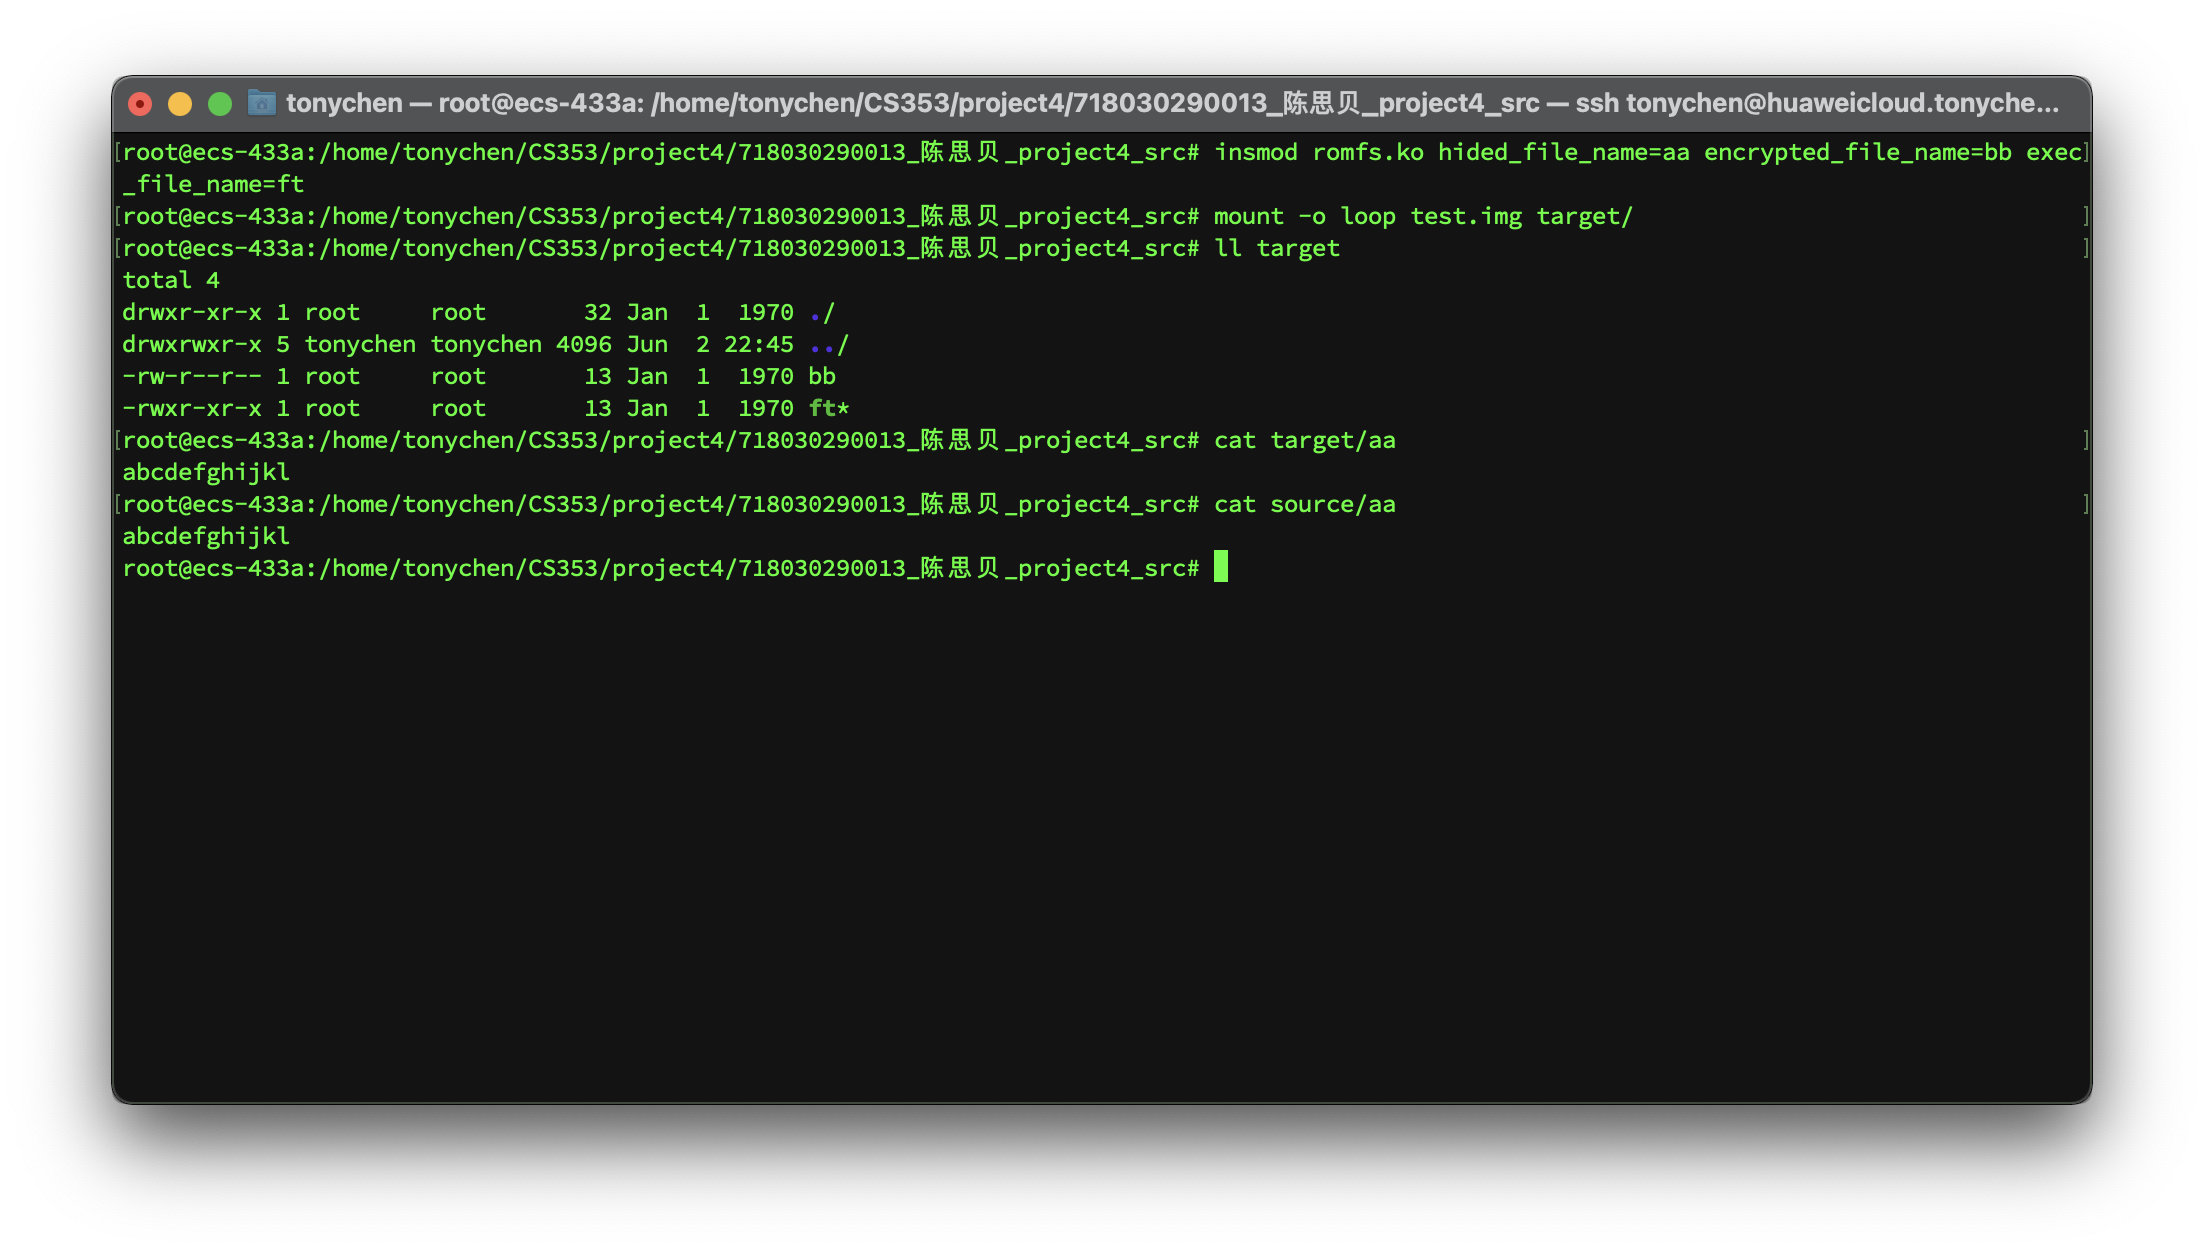
\includegraphics[width=15cm,keepaspectratio]{images/part1.png}
        \caption{隐藏文件效果}
        \label{fig:part1}
    \end{figure}

    \begin{figure}[h!]
        \centering
        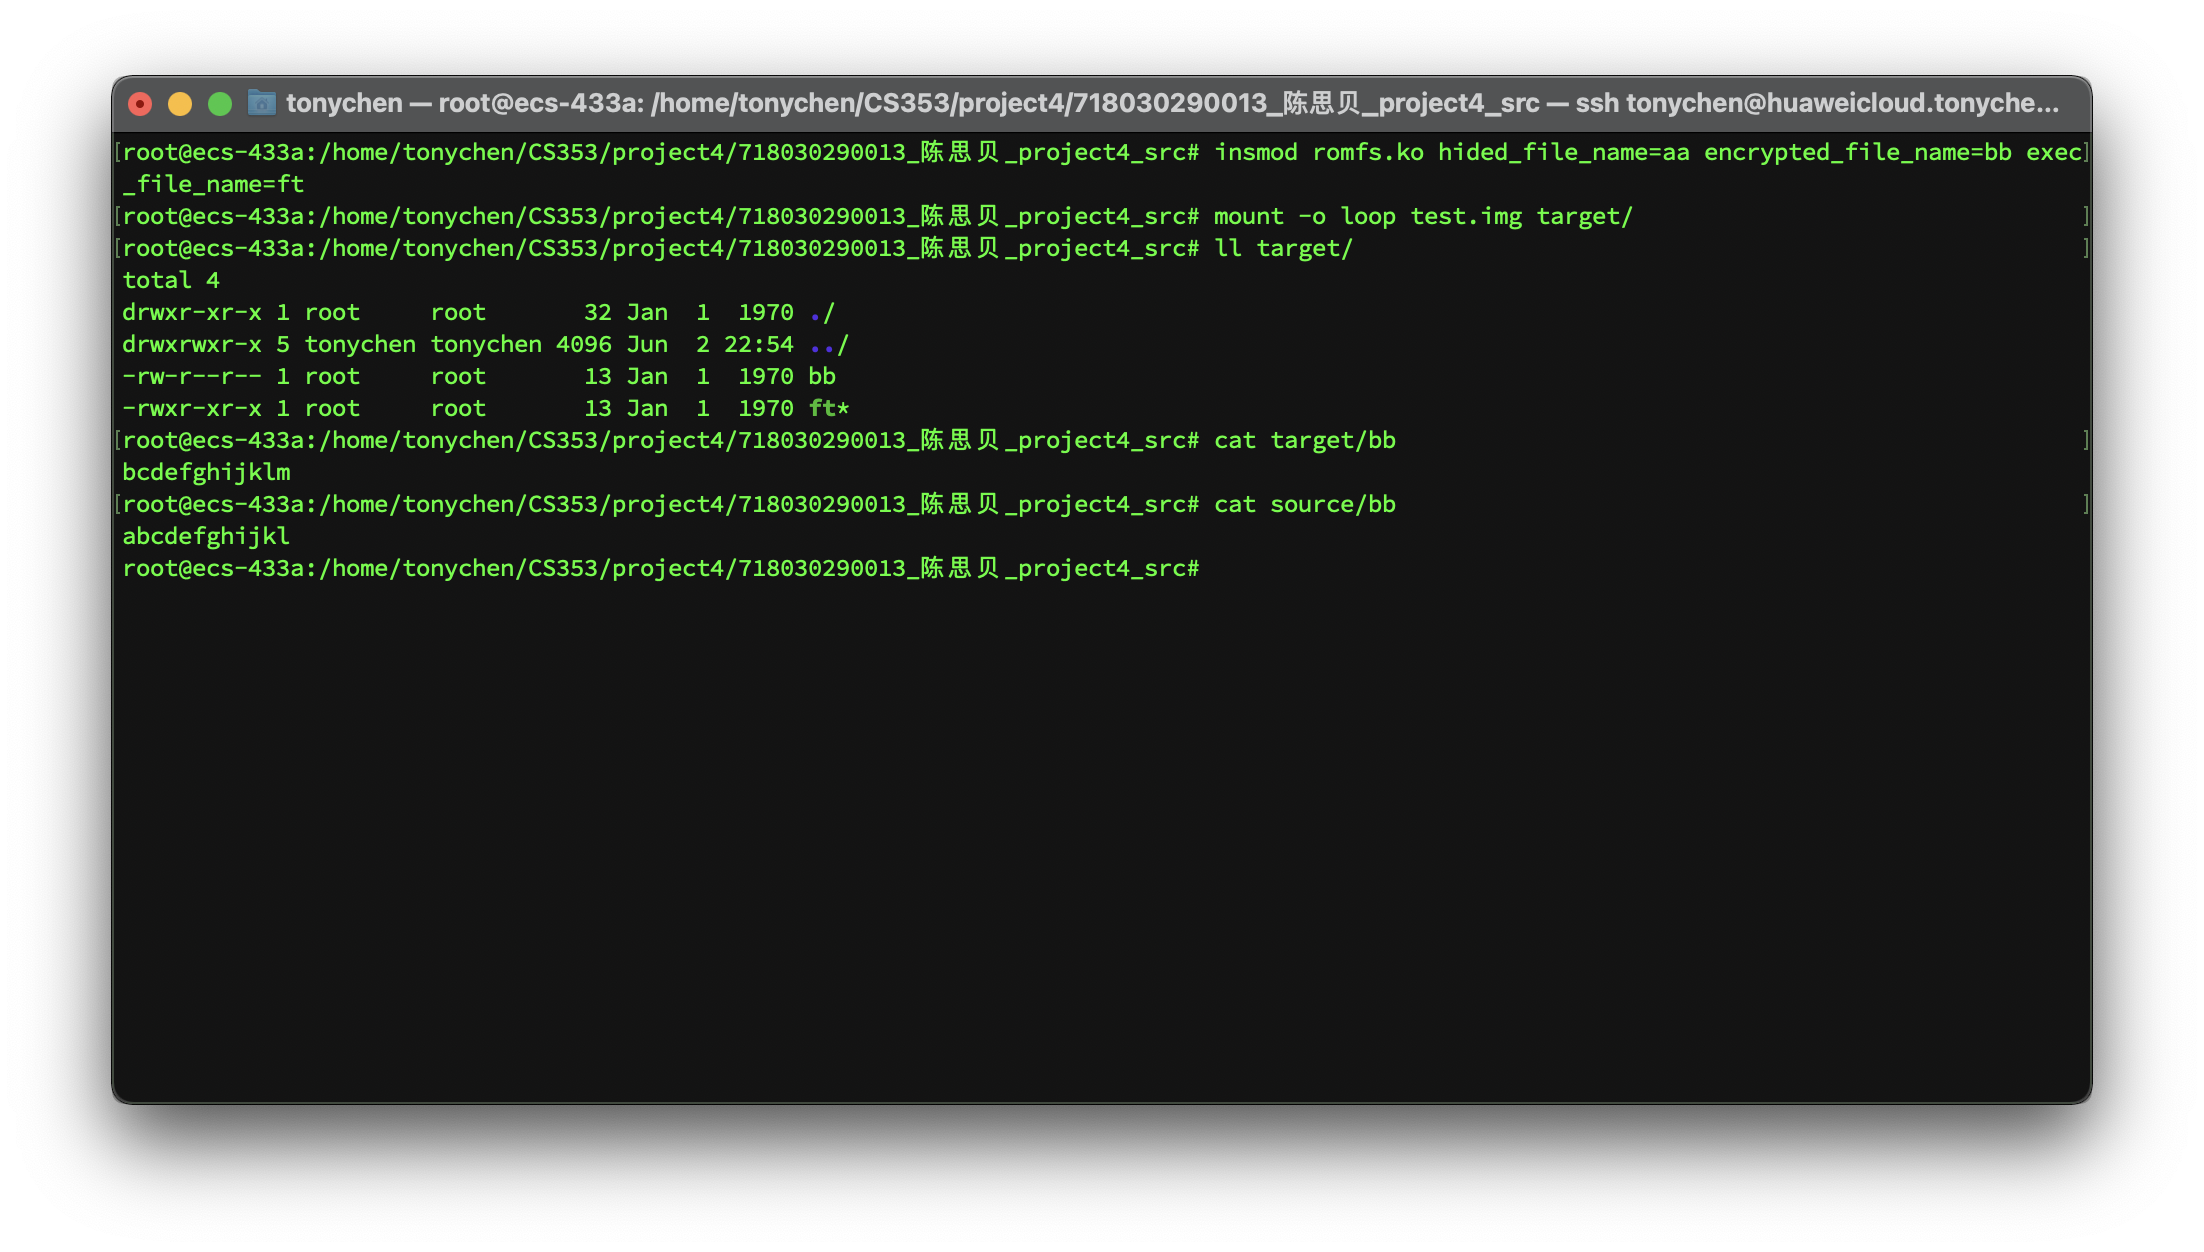
\includegraphics[width=15cm,keepaspectratio]{images/part2.png}
        \caption{加密文件效果}
        \label{fig:part2}
    \end{figure}

    \begin{figure}[h!]
        \centering
        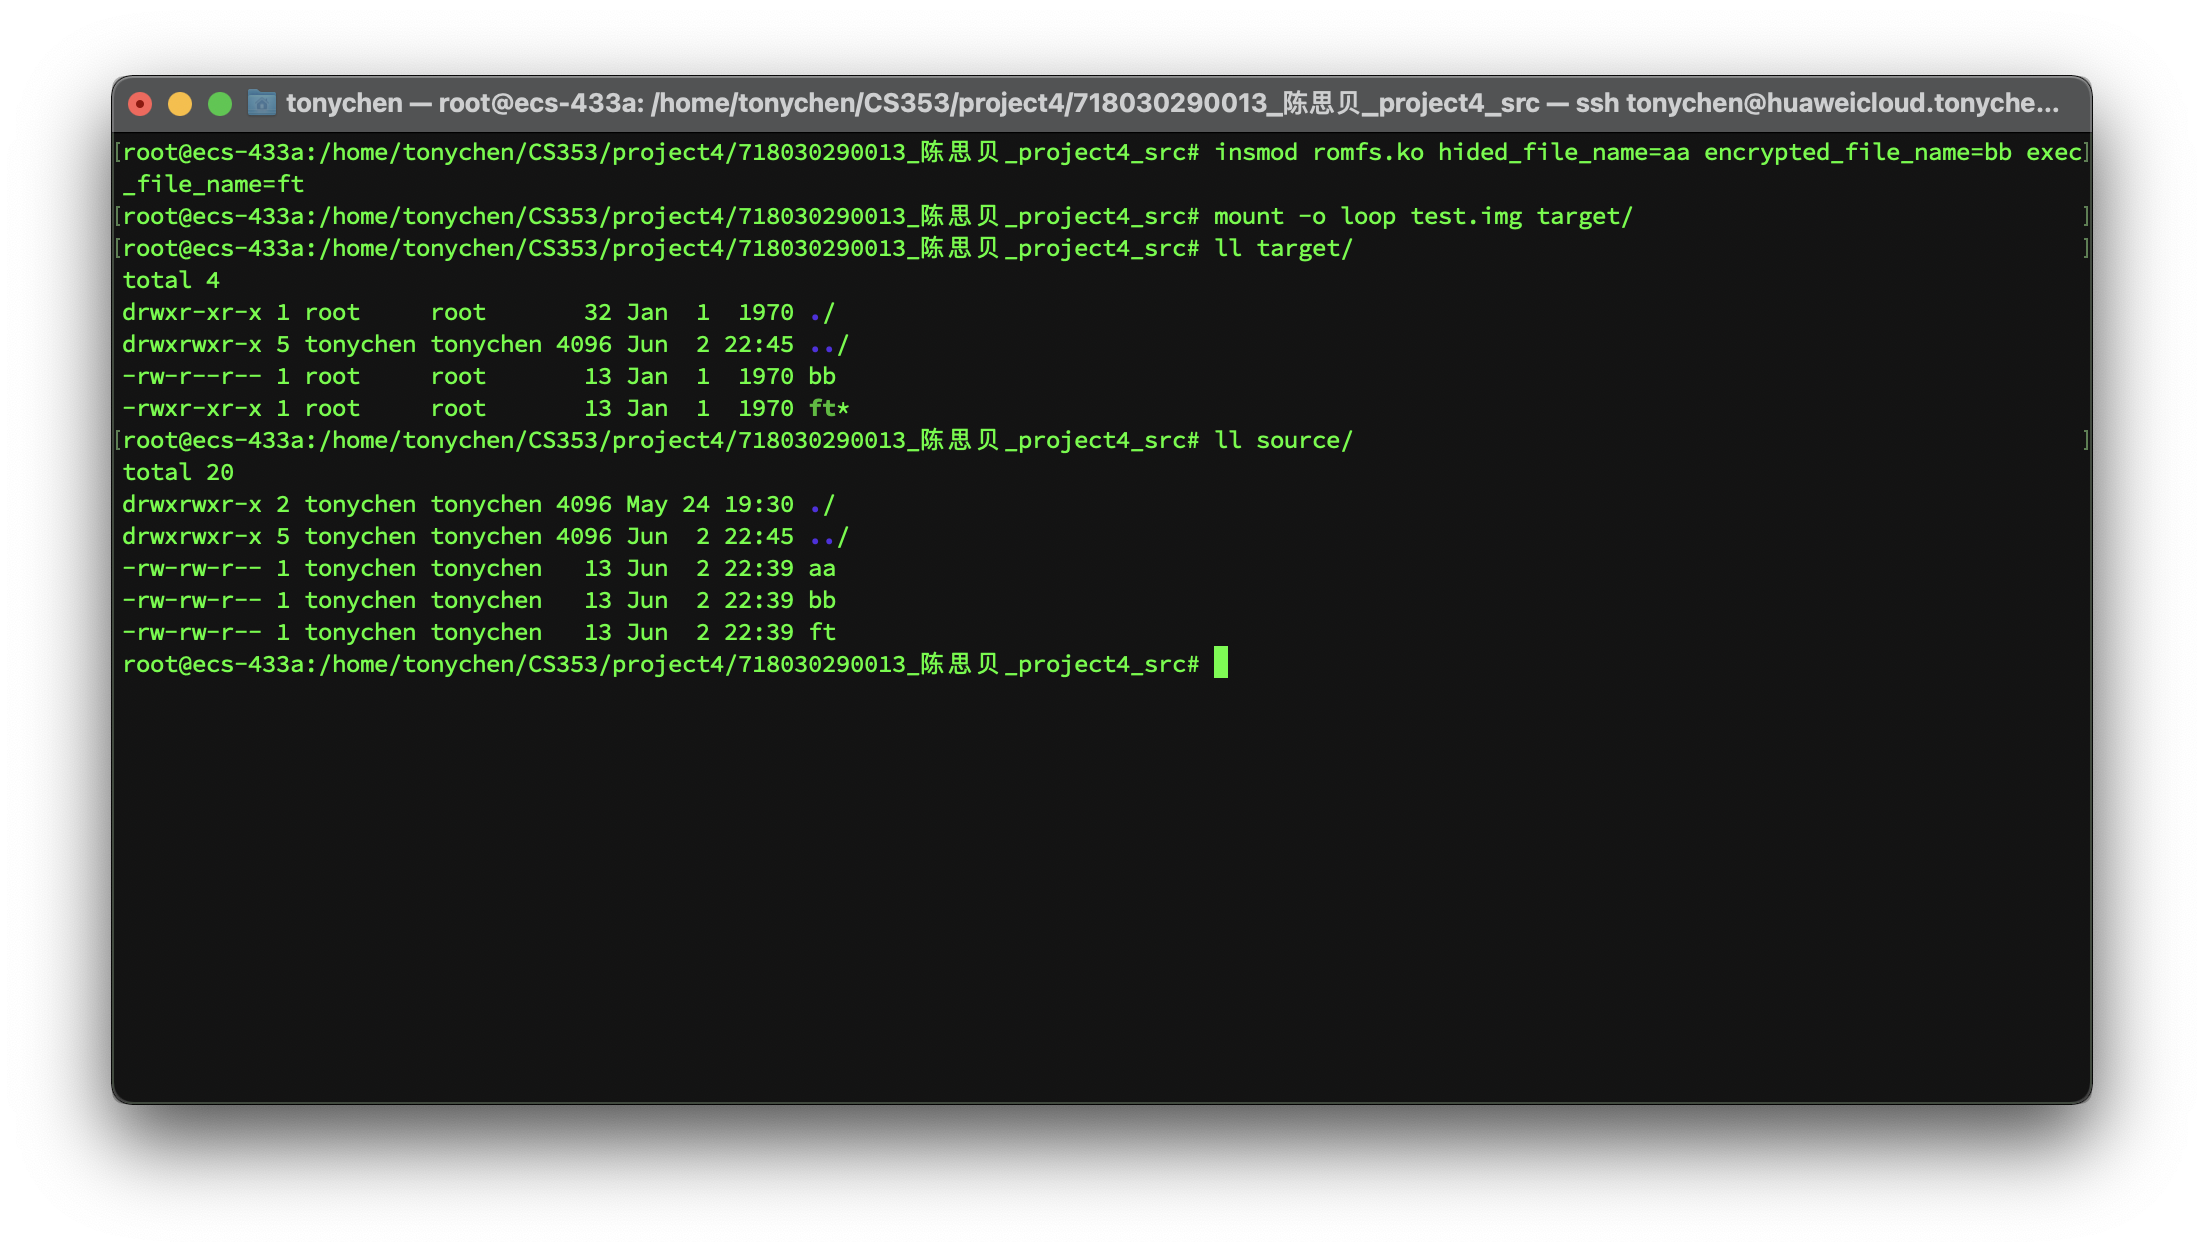
\includegraphics[width=15cm,keepaspectratio]{images/part3.png}
        \caption{修改文件为可执行权限效果}
        \label{fig:part3}
    \end{figure}

    \begin{figure}[h!]
        \centering
        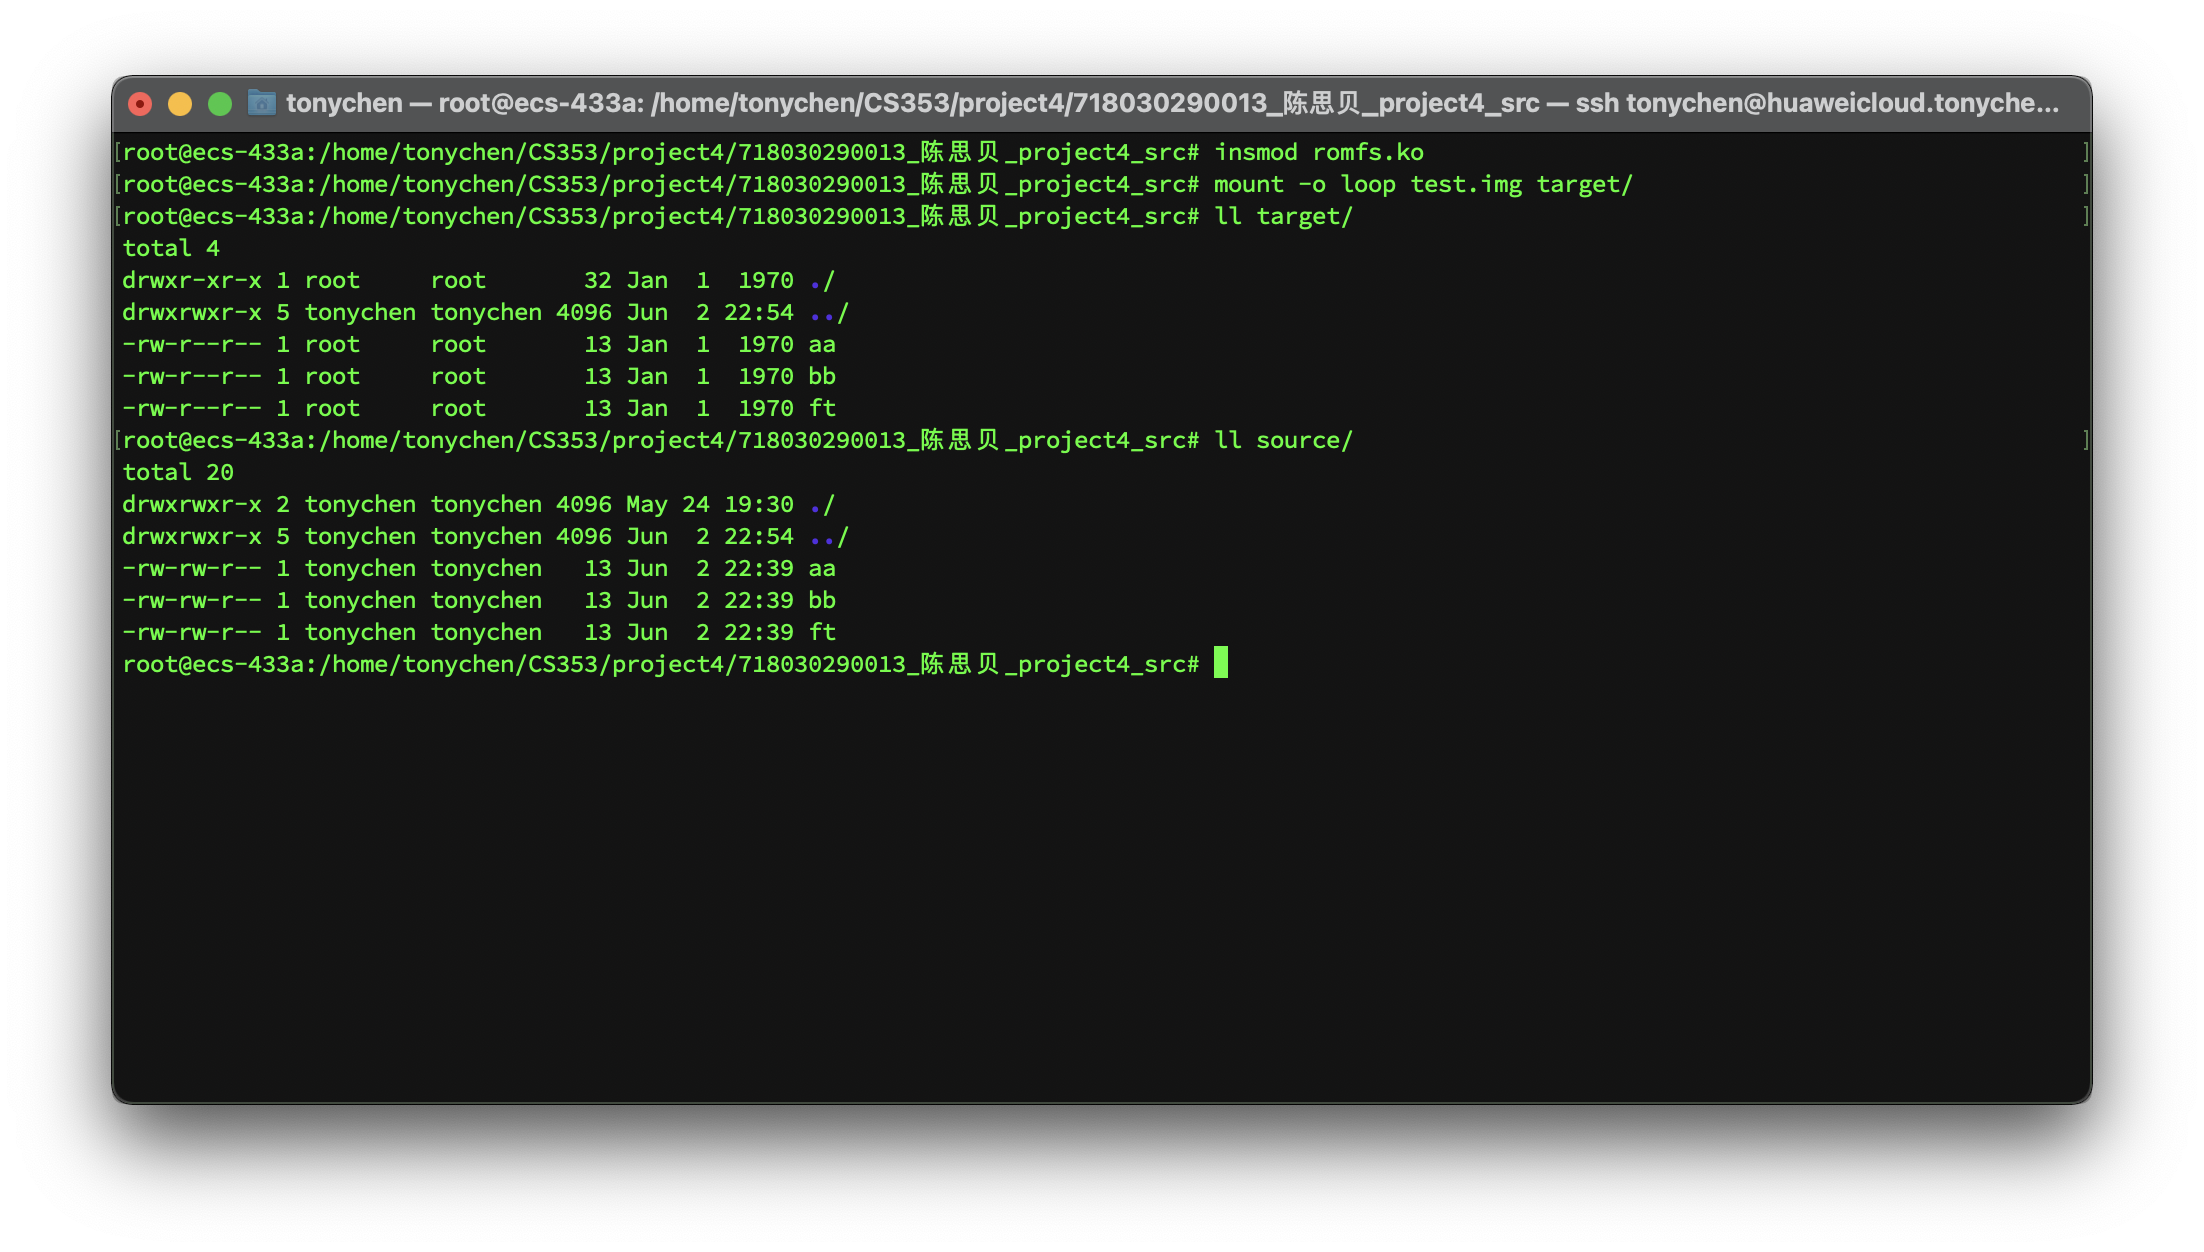
\includegraphics[width=15cm,keepaspectratio]{images/nochg.png}
        \caption{无传参时效果}
        \label{fig:nochg}
    \end{figure}
    

    \section{实验心得}
    通过本次的实验,对Linux中挂载文件系统的\texttt{super.c}有了更深的理解。对于该文件和其他辅助头文件的阅读,对文件管理的操作有了更深的理解。也吸取了前几次实验的教训,对模块特殊情况进行了防呆操作,如不传参数时,\texttt{romfs}模块与未作修改时的模块并无区别(见图\ref{fig:nochg})。

\end{document}